
%% bare_jrnl_comsoc.tex
%% V1.4b
%% 2015/08/26
%% by Michael Shell
%% see http://www.michaelshell.org/
%% for current contact information.
%%
%% This is a skeleton file demonstrating the use of IEEEtran.cls
%% (requires IEEEtran.cls version 1.8b or later) with an IEEE
%% Communications Society journal paper.
%%
%% Support sites:
%% http://www.michaelshell.org/tex/ieeetran/
%% http://www.ctan.org/pkg/ieeetran
%% and
%% http://www.ieee.org/

%%*************************************************************************
%% Legal Notice:
%% This code is offered as-is without any warranty either expressed or
%% implied; without even the implied warranty of MERCHANTABILITY or
%% FITNESS FOR A PARTICULAR PURPOSE! 
%% User assumes all risk.
%% In no event shall the IEEE or any contributor to this code be liable for
%% any damages or losses, including, but not limited to, incidental,
%% consequential, or any other damages, resulting from the use or misuse
%% of any information contained here.
%%
%% All comments are the opinions of their respective authors and are not
%% necessarily endorsed by the IEEE.
%%
%% This work is distributed under the LaTeX Project Public License (LPPL)
%% ( http://www.latex-project.org/ ) version 1.3, and may be freely used,
%% distributed and modified. A copy of the LPPL, version 1.3, is included
%% in the base LaTeX documentation of all distributions of LaTeX released
%% 2003/12/01 or later.
%% Retain all contribution notices and credits.
%% ** Modified files should be clearly indicated as such, including  **
%% ** renaming them and changing author support contact information. **
%%*************************************************************************


% *** Authors should verify (and, if needed, correct) their LaTeX system  ***
% *** with the testflow diagnostic prior to trusting their LaTeX platform ***
% *** with production work. The IEEE's font choices and paper sizes can   ***
% *** trigger bugs that do not appear when using other class files.       ***                          ***
% The testflow support page is at:
% http://www.michaelshell.org/tex/testflow/



\documentclass[journal,comsoc]{IEEEtran}
%
% If IEEEtran.cls has not been installed into the LaTeX system files,
% manually specify the path to it like:
% \documentclass[journal,comsoc]{../sty/IEEEtran}


\usepackage[T1]{fontenc}% optional T1 font encoding


% Some very useful LaTeX packages include:
% (uncomment the ones you want to load)


% *** MISC UTILITY PACKAGES ***
%
%\usepackage{ifpdf}
% Heiko Oberdiek's ifpdf.sty is very useful if you need conditional
% compilation based on whether the output is pdf or dvi.
% usage:
% \ifpdf
%   % pdf code
% \else
%   % dvi code
% \fi
% The latest version of ifpdf.sty can be obtained from:
% http://www.ctan.org/pkg/ifpdf
% Also, note that IEEEtran.cls V1.7 and later provides a builtin
% \ifCLASSINFOpdf conditional that works the same way.
% When switching from latex to pdflatex and vice-versa, the compiler may
% have to be run twice to clear warning/error messages.






% *** CITATION PACKAGES ***
%
%\usepackage{cite}
% cite.sty was written by Donald Arseneau
% V1.6 and later of IEEEtran pre-defines the format of the cite.sty package
% \cite{} output to follow that of the IEEE. Loading the cite package will
% result in citation numbers being automatically sorted and properly
% "compressed/ranged". e.g., [1], [9], [2], [7], [5], [6] without using
% cite.sty will become [1], [2], [5]--[7], [9] using cite.sty. cite.sty's
% \cite will automatically add leading space, if needed. Use cite.sty's
% noadjust option (cite.sty V3.8 and later) if you want to turn this off
% such as if a citation ever needs to be enclosed in parenthesis.
% cite.sty is already installed on most LaTeX systems. Be sure and use
% version 5.0 (2009-03-20) and later if using hyperref.sty.
% The latest version can be obtained at:
% http://www.ctan.org/pkg/cite
% The documentation is contained in the cite.sty file itself.






% *** GRAPHICS RELATED PACKAGES ***
%
\ifCLASSINFOpdf
  % \usepackage[pdftex]{graphicx}
  % declare the path(s) where your graphic files are
  % \graphicspath{{../pdf/}{../jpeg/}}
  % and their extensions so you won't have to specify these with
  % every instance of \includegraphics
  % \DeclareGraphicsExtensions{.pdf,.jpeg,.png}
\else
  % or other class option (dvipsone, dvipdf, if not using dvips). graphicx
  % will default to the driver specified in the system graphics.cfg if no
  % driver is specified.
  % \usepackage[dvips]{graphicx}
  % declare the path(s) where your graphic files are
  % \graphicspath{{../eps/}}
  % and their extensions so you won't have to specify these with
  % every instance of \includegraphics
  % \DeclareGraphicsExtensions{.eps}
\fi
% graphicx was written by David Carlisle and Sebastian Rahtz. It is
% required if you want graphics, photos, etc. graphicx.sty is already
% installed on most LaTeX systems. The latest version and documentation
% can be obtained at: 
% http://www.ctan.org/pkg/graphicx
% Another good source of documentation is "Using Imported Graphics in
% LaTeX2e" by Keith Reckdahl which can be found at:
% http://www.ctan.org/pkg/epslatex
%
% latex, and pdflatex in dvi mode, support graphics in encapsulated
% postscript (.eps) format. pdflatex in pdf mode supports graphics
% in .pdf, .jpeg, .png and .mps (metapost) formats. Users should ensure
% that all non-photo figures use a vector format (.eps, .pdf, .mps) and
% not a bitmapped formats (.jpeg, .png). The IEEE frowns on bitmapped formats
% which can result in "jaggedy"/blurry rendering of lines and letters as
% well as large increases in file sizes.
%
% You can find documentation about the pdfTeX application at:
% http://www.tug.org/applications/pdftex





% *** MATH PACKAGES ***
%
\usepackage{amsmath}
% A popular package from the American Mathematical Society that provides
% many useful and powerful commands for dealing with mathematics.
% Do NOT use the amsbsy package under comsoc mode as that feature is
% already built into the Times Math font (newtxmath, mathtime, etc.).
% 
% Also, note that the amsmath package sets \interdisplaylinepenalty to 10000
% thus preventing page breaks from occurring within multiline equations. Use:
\interdisplaylinepenalty=2500
% after loading amsmath to restore such page breaks as IEEEtran.cls normally
% does. amsmath.sty is already installed on most LaTeX systems. The latest
% version and documentation can be obtained at:
% http://www.ctan.org/pkg/amsmath


% Select a Times math font under comsoc mode or else one will automatically
% be selected for you at the document start. This is required as Communications
% Society journals use a Times, not Computer Modern, math font.
\usepackage[cmintegrals]{newtxmath}
% The freely available newtxmath package was written by Michael Sharpe and
% provides a feature rich Times math font. The cmintegrals option, which is
% the default under IEEEtran, is needed to get the correct style integral
% symbols used in Communications Society journals. Version 1.451, July 28,
% 2015 or later is recommended. Also, do *not* load the newtxtext.sty package
% as doing so would alter the main text font.
% http://www.ctan.org/pkg/newtx
%
% Alternatively, you can use the MathTime commercial fonts if you have them
% installed on your system:
%\usepackage{mtpro2}
%\usepackage{mt11p}
%\usepackage{mathtime}


%\usepackage{bm}
% The bm.sty package was written by David Carlisle and Frank Mittelbach.
% This package provides a \bm{} to produce bold math symbols.
% http://www.ctan.org/pkg/bm





% *** SPECIALIZED LIST PACKAGES ***
%
%\usepackage{algorithmic}
% algorithmic.sty was written by Peter Williams and Rogerio Brito.
% This package provides an algorithmic environment fo describing algorithms.
% You can use the algorithmic environment in-text or within a figure
% environment to provide for a floating algorithm. Do NOT use the algorithm
% floating environment provided by algorithm.sty (by the same authors) or
% algorithm2e.sty (by Christophe Fiorio) as the IEEE does not use dedicated
% algorithm float types and packages that provide these will not provide
% correct IEEE style captions. The latest version and documentation of
% algorithmic.sty can be obtained at:
% http://www.ctan.org/pkg/algorithms
% Also of interest may be the (relatively newer and more customizable)
% algorithmicx.sty package by Szasz Janos:
% http://www.ctan.org/pkg/algorithmicx




% *** ALIGNMENT PACKAGES ***
%
%\usepackage{array}
% Frank Mittelbach's and David Carlisle's array.sty patches and improves
% the standard LaTeX2e array and tabular environments to provide better
% appearance and additional user controls. As the default LaTeX2e table
% generation code is lacking to the point of almost being broken with
% respect to the quality of the end results, all users are strongly
% advised to use an enhanced (at the very least that provided by array.sty)
% set of table tools. array.sty is already installed on most systems. The
% latest version and documentation can be obtained at:
% http://www.ctan.org/pkg/array


% IEEEtran contains the IEEEeqnarray family of commands that can be used to
% generate multiline equations as well as matrices, tables, etc., of high
% quality.




% *** SUBFIGURE PACKAGES ***
%\ifCLASSOPTIONcompsoc
%  \usepackage[caption=false,font=normalsize,labelfont=sf,textfont=sf]{subfig}
%\else
%  \usepackage[caption=false,font=footnotesize]{subfig}
%\fi
% subfig.sty, written by Steven Douglas Cochran, is the modern replacement
% for subfigure.sty, the latter of which is no longer maintained and is
% incompatible with some LaTeX packages including fixltx2e. However,
% subfig.sty requires and automatically loads Axel Sommerfeldt's caption.sty
% which will override IEEEtran.cls' handling of captions and this will result
% in non-IEEE style figure/table captions. To prevent this problem, be sure
% and invoke subfig.sty's "caption=false" package option (available since
% subfig.sty version 1.3, 2005/06/28) as this is will preserve IEEEtran.cls
% handling of captions.
% Note that the Computer Society format requires a larger sans serif font
% than the serif footnote size font used in traditional IEEE formatting
% and thus the need to invoke different subfig.sty package options depending
% on whether compsoc mode has been enabled.
%
% The latest version and documentation of subfig.sty can be obtained at:
% http://www.ctan.org/pkg/subfig




% *** FLOAT PACKAGES ***
%
%\usepackage{fixltx2e}
% fixltx2e, the successor to the earlier fix2col.sty, was written by
% Frank Mittelbach and David Carlisle. This package corrects a few problems
% in the LaTeX2e kernel, the most notable of which is that in current
% LaTeX2e releases, the ordering of single and double column floats is not
% guaranteed to be preserved. Thus, an unpatched LaTeX2e can allow a
% single column figure to be placed prior to an earlier double column
% figure.
% Be aware that LaTeX2e kernels dated 2015 and later have fixltx2e.sty's
% corrections already built into the system in which case a warning will
% be issued if an attempt is made to load fixltx2e.sty as it is no longer
% needed.
% The latest version and documentation can be found at:
% http://www.ctan.org/pkg/fixltx2e


%\usepackage{stfloats}
% stfloats.sty was written by Sigitas Tolusis. This package gives LaTeX2e
% the ability to do double column floats at the bottom of the page as well
% as the top. (e.g., "\begin{figure*}[!b]" is not normally possible in
% LaTeX2e). It also provides a command:
%\fnbelowfloat
% to enable the placement of footnotes below bottom floats (the standard
% LaTeX2e kernel puts them above bottom floats). This is an invasive package
% which rewrites many portions of the LaTeX2e float routines. It may not work
% with other packages that modify the LaTeX2e float routines. The latest
% version and documentation can be obtained at:
% http://www.ctan.org/pkg/stfloats
% Do not use the stfloats baselinefloat ability as the IEEE does not allow
% \baselineskip to stretch. Authors submitting work to the IEEE should note
% that the IEEE rarely uses double column equations and that authors should try
% to avoid such use. Do not be tempted to use the cuted.sty or midfloat.sty
% packages (also by Sigitas Tolusis) as the IEEE does not format its papers in
% such ways.
% Do not attempt to use stfloats with fixltx2e as they are incompatible.
% Instead, use Morten Hogholm'a dblfloatfix which combines the features
% of both fixltx2e and stfloats:
%
% \usepackage{dblfloatfix}
% The latest version can be found at:
% http://www.ctan.org/pkg/dblfloatfix




%\ifCLASSOPTIONcaptionsoff
%  \usepackage[nomarkers]{endfloat}
% \let\MYoriglatexcaption\caption
% \renewcommand{\caption}[2][\relax]{\MYoriglatexcaption[#2]{#2}}
%\fi
% endfloat.sty was written by James Darrell McCauley, Jeff Goldberg and 
% Axel Sommerfeldt. This package may be useful when used in conjunction with 
% IEEEtran.cls'  captionsoff option. Some IEEE journals/societies require that
% submissions have lists of figures/tables at the end of the paper and that
% figures/tables without any captions are placed on a page by themselves at
% the end of the document. If needed, the draftcls IEEEtran class option or
% \CLASSINPUTbaselinestretch interface can be used to increase the line
% spacing as well. Be sure and use the nomarkers option of endfloat to
% prevent endfloat from "marking" where the figures would have been placed
% in the text. The two hack lines of code above are a slight modification of
% that suggested by in the endfloat docs (section 8.4.1) to ensure that
% the full captions always appear in the list of figures/tables - even if
% the user used the short optional argument of \caption[]{}.
% IEEE papers do not typically make use of \caption[]'s optional argument,
% so this should not be an issue. A similar trick can be used to disable
% captions of packages such as subfig.sty that lack options to turn off
% the subcaptions:
% For subfig.sty:
% \let\MYorigsubfloat\subfloat
% \renewcommand{\subfloat}[2][\relax]{\MYorigsubfloat[]{#2}}
% However, the above trick will not work if both optional arguments of
% the \subfloat command are used. Furthermore, there needs to be a
% description of each subfigure *somewhere* and endfloat does not add
% subfigure captions to its list of figures. Thus, the best approach is to
% avoid the use of subfigure captions (many IEEE journals avoid them anyway)
% and instead reference/explain all the subfigures within the main caption.
% The latest version of endfloat.sty and its documentation can obtained at:
% http://www.ctan.org/pkg/endfloat
%
% The IEEEtran \ifCLASSOPTIONcaptionsoff conditional can also be used
% later in the document, say, to conditionally put the References on a 
% page by themselves.




% *** PDF, URL AND HYPERLINK PACKAGES ***
%
%\usepackage{url}
% url.sty was written by Donald Arseneau. It provides better support for
% handling and breaking URLs. url.sty is already installed on most LaTeX
% systems. The latest version and documentation can be obtained at:
% http://www.ctan.org/pkg/url
% Basically, \url{my_url_here}.




% *** Do not adjust lengths that control margins, column widths, etc. ***
% *** Do not use packages that alter fonts (such as pslatex).         ***
% There should be no need to do such things with IEEEtran.cls V1.6 and later.
% (Unless specifically asked to do so by the journal or conference you plan
% to submit to, of course. )


% correct bad hyphenation here
\hyphenation{op-tical net-works semi-conduc-tor}


\usepackage{amsmath}
\usepackage{my_def_env} 
\usepackage{my_def_sym}
\usepackage{graphicx}

\begin{document}
%
% paper title
% Titles are generally capitalized except for words such as a, an, and, as,
% at, but, by, for, in, nor, of, on, or, the, to and up, which are usually
% not capitalized unless they are the first or last word of the title.
% Linebreaks \\ can be used within to get better formatting as desired.
% Do not put math or special symbols in the title.
\title{Inverse Kinematics for 8 Degree of Freedom Robotic System}
%
%
% author names and IEEE memberships
% note positions of commas and nonbreaking spaces ( ~ ) LaTeX will not break
% a structure at a ~ so this keeps an author's name from being broken across
% two lines.
% use \thanks{} to gain access to the first footnote area
% a separate \thanks must be used for each paragraph as LaTeX2e's \thanks
% was not built to handle multiple paragraphs
%

\author{Yuechuan Xue, Xiaoqian Mu}% <-this % stops a space
%\thanks{M. Shell was with the Department
%of Electrical and Computer Engineering, Georgia Institute of Technology, Atlanta,
%GA, 30332 USA e-mail: (see http://www.michaelshell.org/contact.html).}% <-this % stops a space
%\thanks{J. Doe and J. Doe are with Anonymous University.}% <-this % stops a space
%\thanks{Manuscript received April 19, 2005; revised August 26, 2015.}

% note the % following the last \IEEEmembership and also \thanks - 
% these prevent an unwanted space from occurring between the last author name
% and the end of the author line. i.e., if you had this:
% 
% \author{....lastname \thanks{...} \thanks{...} }
%                     ^------------^------------^----Do not want these spaces!
%
% a space would be appended to the last name and could cause every name on that
% line to be shifted left slightly. This is one of those "LaTeX things". For
% instance, "\textbf{A} \textbf{B}" will typeset as "A B" not "AB". To get
% "AB" then you have to do: "\textbf{A}\textbf{B}"
% \thanks is no different in this regard, so shield the last } of each \thanks
% that ends a line with a % and do not let a space in before the next \thanks.
% Spaces after \IEEEmembership other than the last one are OK (and needed) as
% you are supposed to have spaces between the names. For what it is worth,
% this is a minor point as most people would not even notice if the said evil
% space somehow managed to creep in.



% The paper headers
%\markboth{Journal of \LaTeX\ Class Files,~Vol.~14, No.~8, August~2015}%
%{Shell \MakeLowercase{\textit{et al.}}: Bare Demo of IEEEtran.cls for IEEE Communications Society Journals}
% The only time the second header will appear is for the odd numbered pages
% after the title page when using the twoside option.
% 
% *** Note that you probably will NOT want to include the author's ***
% *** name in the headers of peer review papers.                   ***
% You can use \ifCLASSOPTIONpeerreview for conditional compilation here if
% you desire.




% If you want to put a publisher's ID mark on the page you can do it like
% this:
%\IEEEpubid{0000--0000/00\$00.00~\copyright~2015 IEEE}
% Remember, if you use this you must call \IEEEpubidadjcol in the second
% column for its text to clear the IEEEpubid mark.



% use for special paper notices
%\IEEEspecialpapernotice{(Invited Paper)}




% make the title area
\maketitle

% As a general rule, do not put math, special symbols or citations
% in the abstract or keywords.
\begin{abstract}
Robotic kinematic describes the nonlinear relationship between the joint space and task space. Solving the inverse kinematics problem is finding the joints variables that corresponds to the task space positions. Usually, it's hard to solve the inverse kinematics for a multi degree of freedom robot system since it's a nonlinear problem with multiple variables as well as constraints from both the joint limits and task specifications. Considered about the complexity of this problem, the nonlinear optimization algorithm becomes a perfect choice in general cases. 
\end{abstract}

% Note that keywords are not normally used for peerreview papers.
\begin{IEEEkeywords}
Inverse Kinematics, Robotics, Nonlinear optimization, Sequential Quadratic Programming(SQP).
\end{IEEEkeywords}






% For peer review papers, you can put extra information on the cover
% page as needed:
% \ifCLASSOPTIONpeerreview
% \begin{center} \bfseries EDICS Category: 3-BBND \end{center}
% \fi
%
% For peerreview papers, this IEEEtran command inserts a page break and
% creates the second title. It will be ignored for other modes.
\IEEEpeerreviewmaketitle



\section{Introduction}
% The very first letter is a 2 line initial drop letter followed
% by the rest of the first word in caps.
% 
% form to use if the first word consists of a single letter:
% \IEEEPARstart{A}{demo} file is ....
% 
% form to use if you need the single drop letter followed by
% normal text (unknown if ever used by the IEEE):
% \IEEEPARstart{A}{}demo file is ....
% 
% Some journals put the first two words in caps:
% \IEEEPARstart{T}{his demo} file is ....
% 
% Here we have the typical use of a "T" for an initial drop letter
% and "HIS" in caps to complete the first word.
\IEEEPARstart{I}{nverse} kinematics is one of the fundamental problems in robotics research which objective is to find a robot configuration that leads the robot end effector to desired position and orientation within the limits of the robot manipulator.In other words, inverse kinematics transfers the end effector task space coordinates into joint space coordinates. The position and orientation of the end effector are nonlinearly related to the joint variables which number is the DOF of the robot. \\

In three-dimensional space, a manipulator with six or more DOF is able to attain any end effector position and  orientation. If the manipulator has six DOF, the system with six nonlinear equations can be solved for six joint variables. However, if the robot manipulator has more than six DOF, it is underdetermined since it has more variable than equations. The inverse kinematics problem can be treated as a root finding problem of multi-variables nonlinear polynomial equations. Unfortunately, it is hard to find the analytical solution. \\

Numerical methods like the Newton-Raphsom(NR) method can be used to solve inverse kinematics problem. The NR method can find solutions if and only if the Jacobian matrix is always reversible and the equations are solvable. The former condition means that the robot should be nonredundant, namely, the number of variables should be the same as the number of equations and constraints, and the robot will not pass through the singular points during moving from the initial configuration to the final configuration. The latter one means the destination position and orientation for the end effector should within the workspace of the robot manipulator. \\ 

Usually, the inverse kinematics problem should be considered under the task for robot manipulator. The specification of the robot task will introduce addtional constraints for this problem which make  it much more complex. Nonlinear optimization algorithms become a good choice for solving inverse kinematics. \\

The organization of this report is as follows: The kinematics problem is introduced in Section II. Section III presents the formulation of eight DOF inverse kinematics problem for grasping objects. Section IV shows the principles of SQP algorithm. Simulation result and discussions are  in Section V.  

% You must have at least 2 lines in the paragraph with the drop letter
% (should never be an issue)



\section{ROBOT KINEMATICS}
Kinematics treats motion of robot manipulator without considering the forces cause it. Within kinematics, the relationship between position, velocity, acceleration and all higher order derivatives of the position variables can be studied. In other words, kinematics of robot manipulators refers to all the geometrical and time-based properties of the motion. \\

Inverse kinematics is given a desired position in the world frame solving for the joint variables . Since the relationship between joint variables and the position if nonlinear and the number of variables is more then the equations in the relationship, it's impossible to solve the inverse kinematics problem directly. \\

In kinematics, the transformation matrix $\Tb$ is necessary, 
\[
\begin{split}
\Tb &= 
  \left[
  \begin{matrix}
  \Rb & \db \\
  \mbox{\boldmath $0$}& 1	
  \end{matrix}	
  \right] \\
  &=
  \left[
  \begin{matrix}
  r_{11} & r_{12} & r_{13} & d_1 \\
  r_{21} & r_{22} & r_{23} & d_2 \\
  r_{31} & r_{32} & r_{33} & d_3 \\
  0 & 0 & 0 & 1	
  \end{matrix} 
  \right] 
  \end{split} \tag{1}
\] 
in which $\Rb$ is the rotation matrix and $\db$ is the transition vector. Elements in $\Rb$ and $\db$ are decided by the joint variables of the robot manipulator. Let $\Theta = (\theta_1, \theta_2, ..., \theta_n)$ be the joint variable vector. We can rewrite $\Rb$,$\db$ and $\Tb$ as $\Rb(\Theta)$,$\db(\Theta)$ and $\Tb(\Theta)$.  \\

Robot manipulator is multiple joints system.  To calculate the position of the end effector in the world frame, local frame system for joints should be created and each joint has one aligned local frame.
 The first frame is the world/base frame and $\Tb_i^{i+1}$ is the transformation matrix from the $i$th frame to $i+1$th frame.  Then we have 
\[
\pb_w = \Tb_0^1*\Tb_1^2*... *\Tb_{n-1}^n * \pb_e \tag{2}
\]
 in which $\pb_w$ is the position of one point in the world frame, $\pb_e$ is the position in the end effector's local frame and $n$ is the degree of freedom of the robot system.\\

Our robot system contains one four DOF robot arm and one four DOF robot hand. So the system's DOF is eight. The robot system and it's model with local frames are shown in Fig 1. 
 
\begin{figure}[!t]
\centering
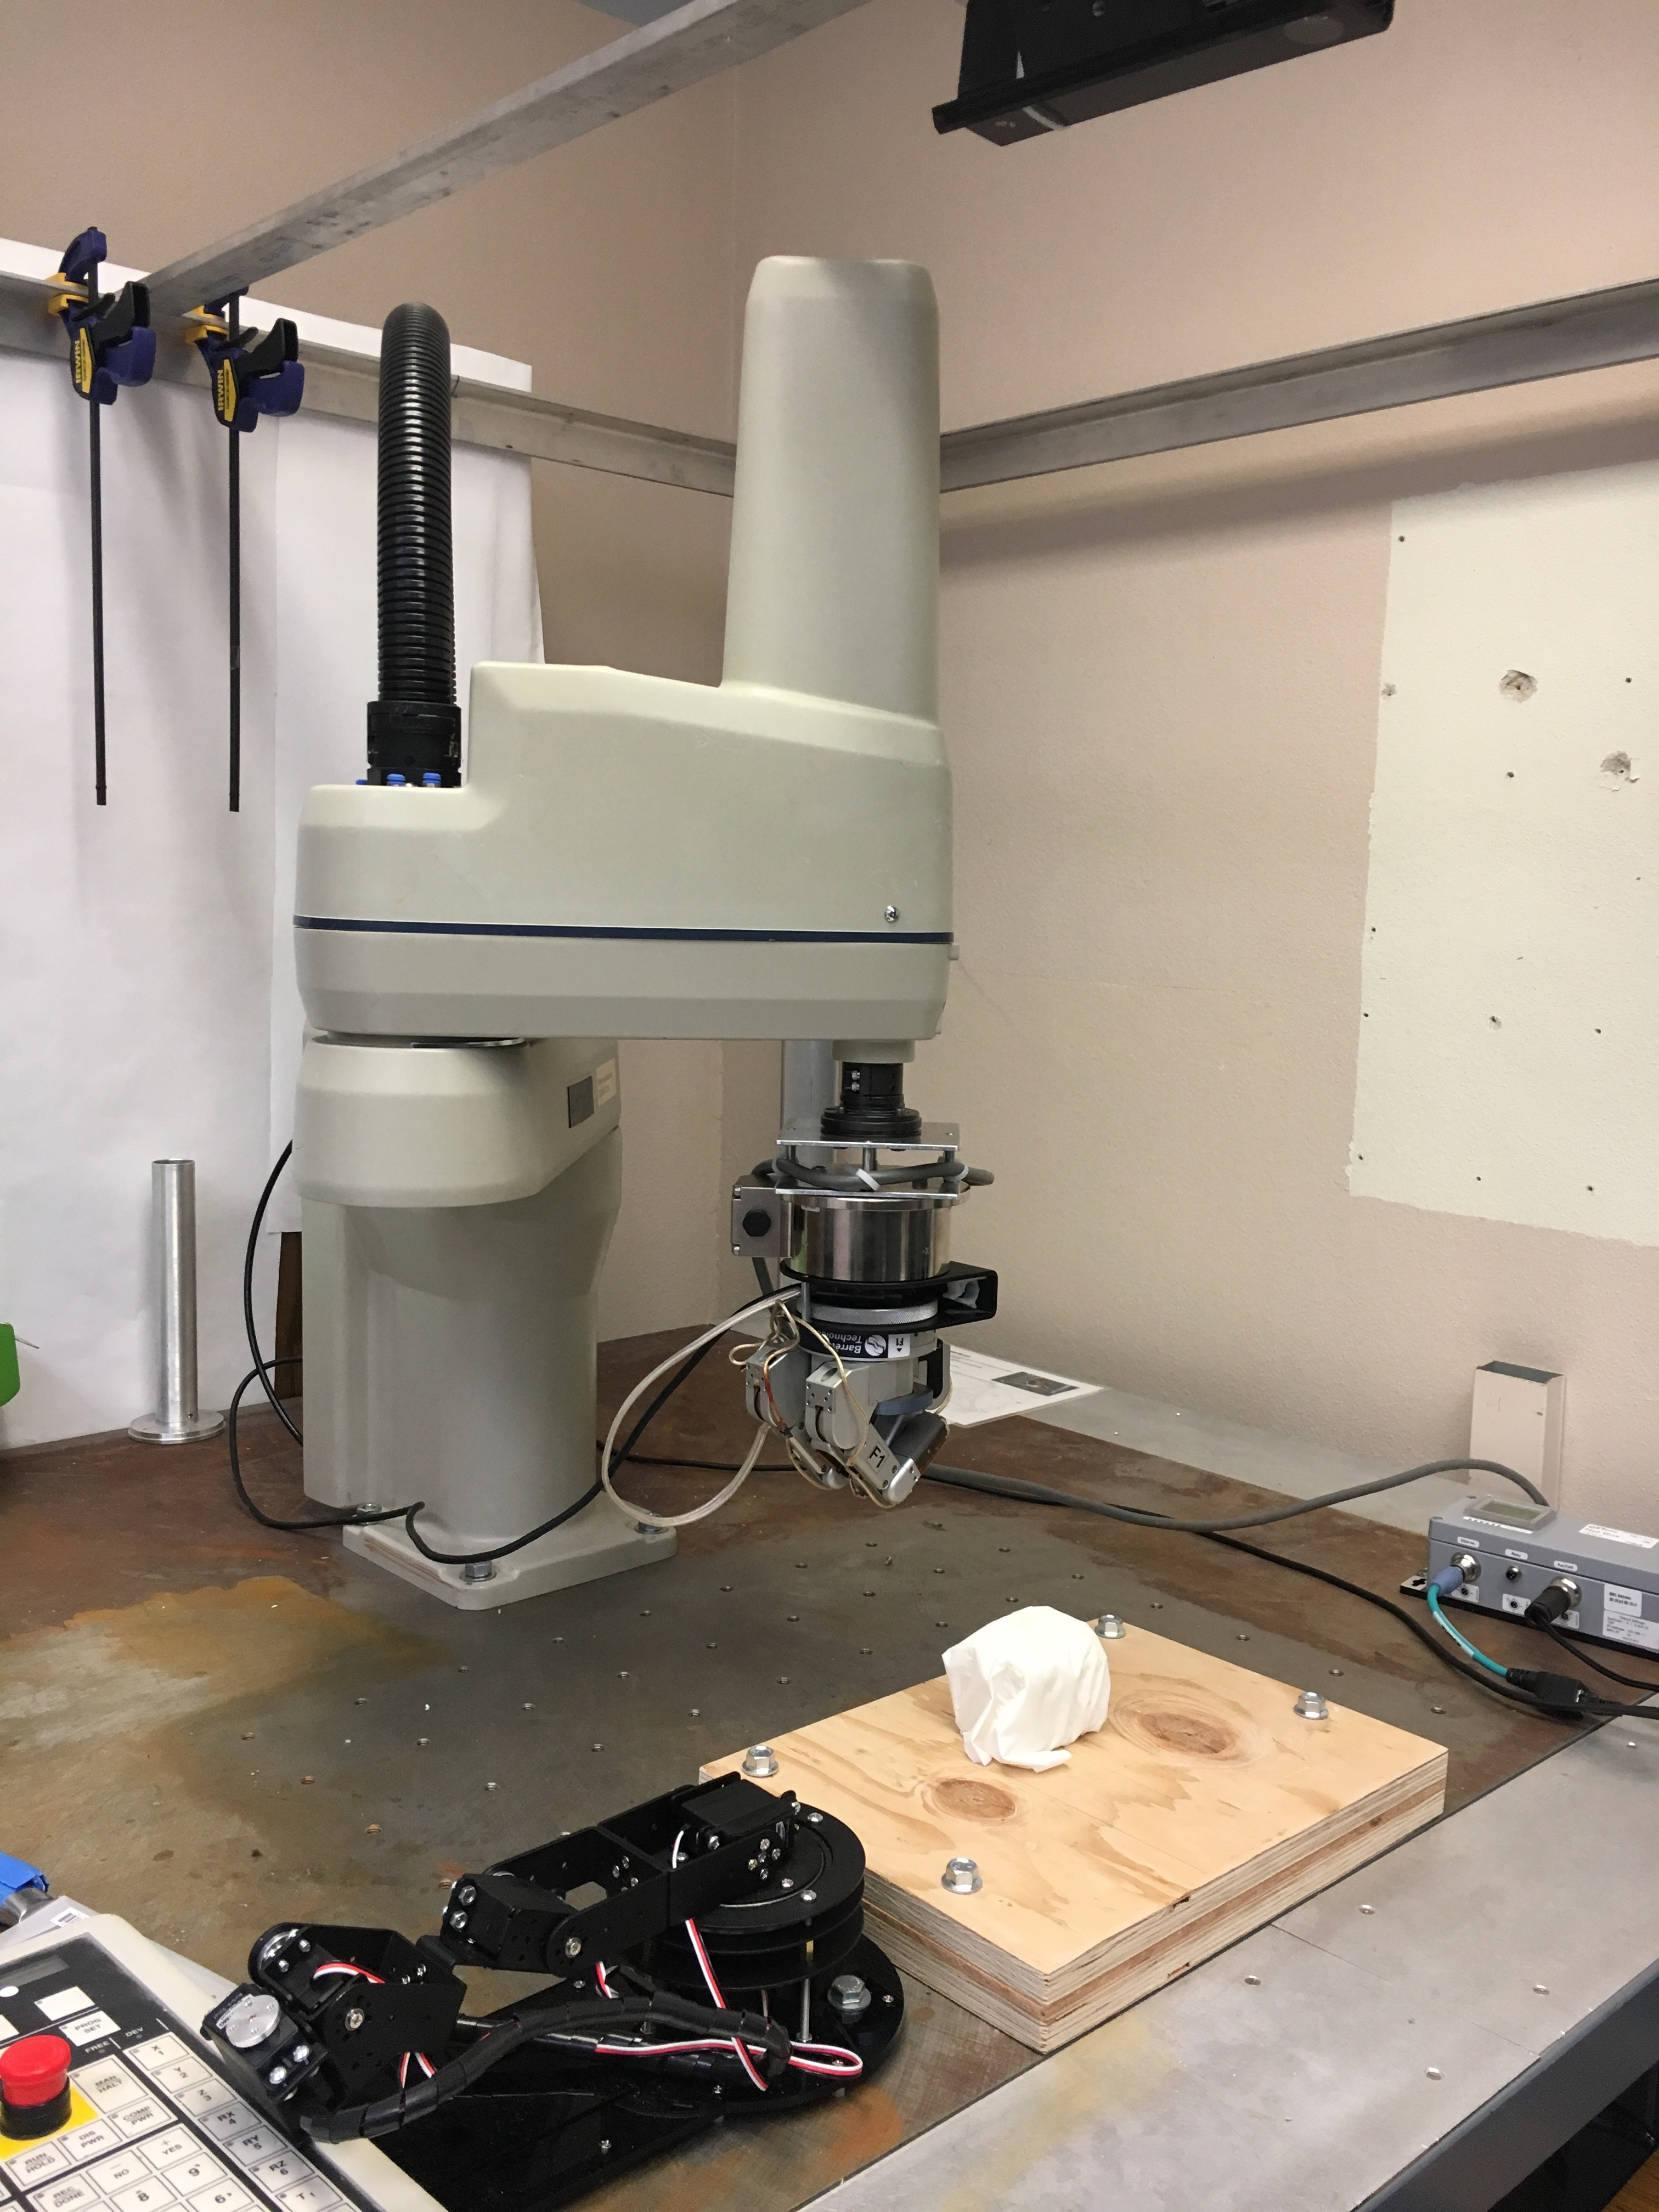
\includegraphics[width=1.5in, height=2.0in]{IMG_5860.jpg}
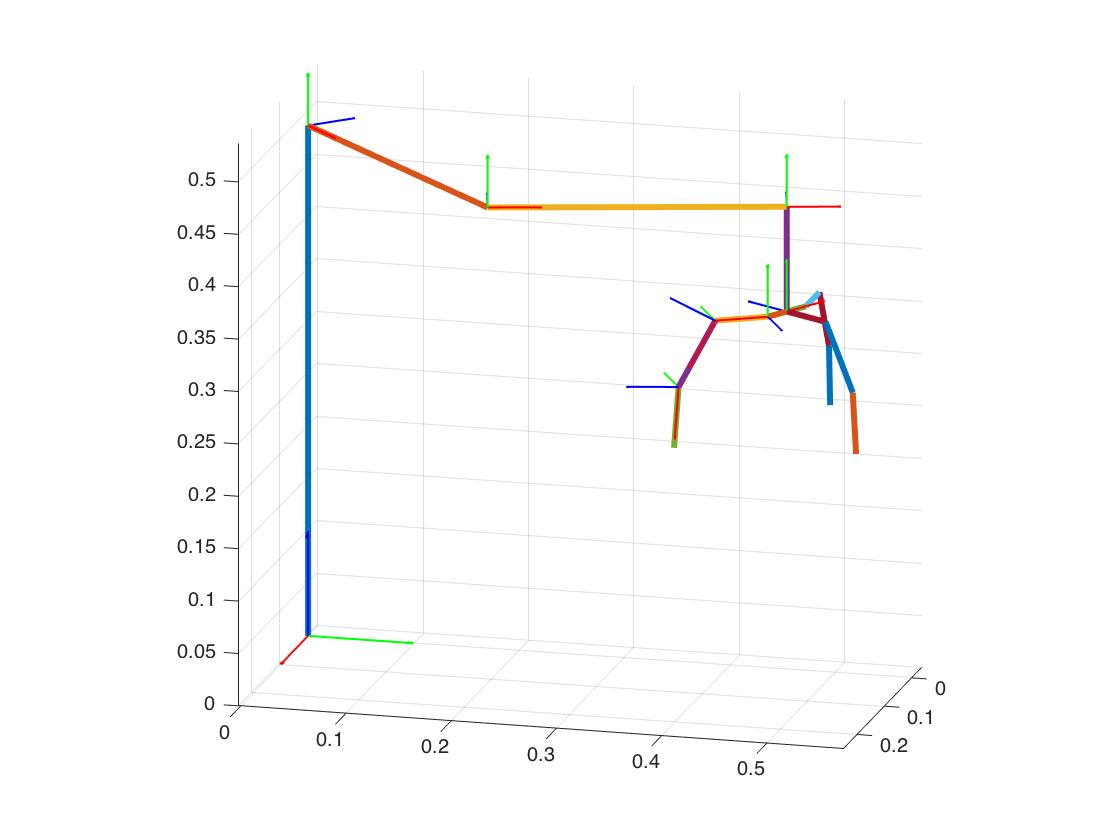
\includegraphics[width=2.5in]{frames.jpg}
\caption{Frame system for the robot manipulator with red line as x direction, green line as y direction and blue line as z direction. }
\label{fig_sim }
\end{figure}

 

\section{PROBLEM FORMULATION}
Inverse kinematics usually comes with  specific robot tasks.  So when we try to solve this problem, it is necessary to consider the task constraints. Moreover, robot has it's own workspace, which also can introduce limitations for the inverse kinematics problem. \\ 

Consider the grasping task for robot manipulator, which requires the robot's fingers reach desired positions on the surface of the object. This problem can be described as follows:
\begin{itemize} 
\item All the joint variables should be within the limits of the robot joints
\item The target points should be located on the lower links of the robot fingers
\item The lower links should be parallel to the tangential plane of the target points
\end{itemize} 

The first characteristic means that the solution should be reasonable. If the joints variables are out of the boundary, the robot can't achieve such configuration and the solution is meaningless. The second property comes form the grasping experiment of human beings since we prefer to use the tip part of our hand rather than the plum to grasp objects. The third one regulate the grasping task by guaranteeing the fingers will not insert into the object. \\

The nonlinearity  together with multiple constraints make the inverse kinematics problem much more complex. We can convert it into a nonlinear optimization problem as follows: 
\[
\min \ \  \sum_{i=0}^{2} \frac{\|(\pb_i-\qb_{i1})\times (\pb_i-\qb_{i2}) \|}{\|\qb_i-\qb_{i2}\|}   \tag{3}
\]

Subject to 
\[
\nb_i \times \lb_{\perp i} =0 \tag{4}
\]
\[
\nb_i * \lb_{\perp i} \geq 0    \tag{5}
\]
\[
 t_i* \qb_{i1} +(1-t_i) * \qb_{i2} = \pb_i  \tag{6}
\]
\[
lb_i \leq \theta_i \leq ub_i  \ \ \ \     i=0, 1, ..., 7  \tag{7}
\]
\[
0 \leq t_i  \leq 1    \ \ \ \     i=0, 1, 2   \tag{8}
\]

In the objective function which minimize the sum of distance from the target points to the lower links, $\pb_i$ is the $i$th target point, $\qb_{i1}$ is the top point of $i$th lower link and $\qb_{i2}$  is the tip of $i$th lower link. $\nb_i$ is the normal direction of the tangential plane of $i$th target point and $\lb_{\perp i}$ is the normal direction of the $i$th lower link.\\ Equation (4) guarantees the normal direction of the lower links parallel to the normal directions of the tangential planes which means the lower links parallel to the tangential planes. Inequality (5) shows that the angles between the normal directions of the lower links and  normal directions of tangential planes  are less than $\pi$. (4) and (5) together make sure that the normal vectors are in the same direction. \\


Equation (6) and (8) mean that $\pb_i$ is on the segment with two end points $\qb_{i1}$ and $\qb_{i2}$. For the inverse kinematics problem, it corresponding to the target points should be on the lower links of the robot hand. (7) gives the mechanical limits of the robot manipulator. In other words, it defines the workspace of the robot. \\



 
% needed in second column of first page if using \IEEEpubid
%\IEEEpubidadjcol




% An example of a floating figure using the graphicx package.
% Note that \label must occur AFTER (or within) \caption.
% For figures, \caption should occur after the \includegraphics.
% Note that IEEEtran v1.7 and later has special internal code that
% is designed to preserve the operation of \label within \caption
% even when the captionsoff option is in effect. However, because
% of issues like this, it may be the safest practice to put all your
% \label just after \caption rather than within \caption{}.
%
% Reminder: the "draftcls" or "draftclsnofoot", not "draft", class
% option should be used if it is desired that the figures are to be
% displayed while in draft mode.
%
%\begin{figure}[!t]
%\centering
%\includegraphics[width=2.5in]{myfigure}
% where an .eps filename suffix will be assumed under latex, 
% and a .pdf suffix will be assumed for pdflatex; or what has been declared
% via \DeclareGraphicsExtensions.
%\caption{Simulation results for the network.}
%\label{fig_sim}
%\end{figure}

% Note that the IEEE typically puts floats only at the top, even when this
% results in a large percentage of a column being occupied by floats.


% An example of a double column floating figure using two subfigures.
% (The subfig.sty package must be loaded for this to work.)
% The subfigure \label commands are set within each subfloat command,
% and the \label for the overall figure must come after \caption.
% \hfil is used as a separator to get equal spacing.
% Watch out that the combined width of all the subfigures on a 
% line do not exceed the text width or a line break will occur.
%
%\begin{figure*}[!t]
%\centering
%\subfloat[Case I]{\includegraphics[width=2.5in]{box}%
%\label{fig_first_case}}
%\hfil
%\subfloat[Case II]{\includegraphics[width=2.5in]{box}%
%\label{fig_second_case}}
%\caption{Simulation results for the network.}
%\label{fig_sim}
%\end{figure*}
%
% Note that often IEEE papers with subfigures do not employ subfigure
% captions (using the optional argument to \subfloat[]), but instead will
% reference/describe all of them (a), (b), etc., within the main caption.
% Be aware that for subfig.sty to generate the (a), (b), etc., subfigure
% labels, the optional argument to \subfloat must be present. If a
% subcaption is not desired, just leave its contents blank,
% e.g., \subfloat[].


% An example of a floating table. Note that, for IEEE style tables, the
% \caption command should come BEFORE the table and, given that table
% captions serve much like titles, are usually capitalized except for words
% such as a, an, and, as, at, but, by, for, in, nor, of, on, or, the, to
% and up, which are usually not capitalized unless they are the first or
% last word of the caption. Table text will default to \footnotesize as
% the IEEE normally uses this smaller font for tables.
% The \label must come after \caption as always.
%
%\begin{table}[!t]
%% increase table row spacing, adjust to taste
%\renewcommand{\arraystretch}{1.3}
% if using array.sty, it might be a good idea to tweak the value of
% \extrarowheight as needed to properly center the text within the cells
%\caption{An Example of a Table}
%\label{table_example}
%\centering
%% Some packages, such as MDW tools, offer better commands for making tables
%% than the plain LaTeX2e tabular which is used here.
%\begin{tabular}{|c||c|}
%\hline
%One & Two\\
%\hline
%Three & Four\\
%\hline
%\end{tabular}
%\end{table}


% Note that the IEEE does not put floats in the very first column
% - or typically anywhere on the first page for that matter. Also,
% in-text middle ("here") positioning is typically not used, but it
% is allowed and encouraged for Computer Society conferences (but
% not Computer Society journals). Most IEEE journals/conferences use
% top floats exclusively. 
% Note that, LaTeX2e, unlike IEEE journals/conferences, places
% footnotes above bottom floats. This can be corrected via the
% \fnbelowfloat command of the stfloats package.

\section{Sequential Quadratic Programming}

In constrained optimization, the general aim is to transform the problem into an easier subproblem that can then be solved and used as the basis of an iterative process. A characteristic of a large class of early methods is the translation of the constrained problem to a basic unconstrained problem by using a penalty function for constraints that are near or beyond the constraint boundary. In this way the constrained problem is solved using a sequence of parameterized unconstrained optimizations, which in the limit (of the sequence) converge to the constrained problem. These methods are now considered relatively inefficient and have been replaced by methods that have focused on the solution of the Karush-Kuhn-Tucker (KKT) equations. The KKT equations are necessary conditions for optimality for a constrained optimization problem. If the problem is a so-called convex programming problem, that is, $f(x)$ and $g_i(x)$, $i = 1,\cdots,m$, are convex functions, then the KKT equations are both necessary and sufficient for a global solution point.

The Kuhn-Tucker equations can be stated as

\begin{equation}
	\min f(x)
\end{equation}

subject to 
\begin{eqnarray}
	g_i(x) & = & 0, \quad i = 1, \cdots , m_e\\
	g_i(x) & \leq & 0, \quad i = m_e+1, \cdots, m \\
	\nabla f(\xb^*) + \sum_{i=1}^m \lambda_i \cdot \nabla g_i(\xb^*) & = & 0 \label{eq:kkt-gradient}\\
	\lambda_i \cdot g_i(\xb^*) & = & 0, \quad i = 1, \cdots , m_e\\
	\lambda_i & \geq & 0, \quad  i = m_e+1, \cdots, m
\end{eqnarray}

The equation (\ref{eq:kkt-gradient}) describes a canceling of the gradients between the objective function and the active constraints at the solution point. For the gradients to be canceled, Lagrange multipliers ($\lambda_i, i = 1,\cdots,m$) are necessary to balance the deviations in magnitude of the objective function and constraint gradients. Because only active constraints are included in this canceling operation, constraints that are not active must not be included in this operation and so are given Lagrange multipliers equal to 0. This is stated implicitly in the last two Kuhn-Tucker equations.

The solution of the KKT equations forms the basis to many nonlinear programming algorithms. These algorithms attempt to compute the Lagrange multipliers directly. Constrained quasi-Newton methods guarantee superlinear convergence by accumulating second-order information regarding the KKT equations using a quasi-Newton updating procedure. These methods are commonly referred to as Sequential Quadratic Programming (SQP) methods, since a QP subproblem is solved at each major iteration (also known as Iterative Quadratic Programming, Recursive Quadratic Programming, and Constrained Variable Metric methods).

\subsection{Active Set Method}

 Active Set method allows to closely mimic Newton's method for constrained optimization just as is done for unconstrained optimization. At each major iteration, an approximation is made of the Hessian of the Lagrangian function using a quasi-Newton updating method. This is then used to generate a QP subproblem whose solution is used to form a search direction for a line search procedure. 
 
\subsection{Quadratic Subproblem}

\begin{equation}
	\min {1 \over 2} \db^\top H_k \db + \nabla f(\xb_k)^\top \db
\end{equation}
subject to:
\begin{eqnarray}
	\nabla g_i(\xb_k)^\top \db + g_i(\xb_k) & = & 0	, \quad i = 1,\cdots , m_e \\
	\nabla g_i(\xb_k)^\top \db + g_i(\xb_k) & \leq & 0	, \quad i = m_e + 1,\cdots , m
\end{eqnarray}
This subproblem can be solved using any QP algorithm. The solution is used to form a new iterate
\begin{equation}
	\xb_{k+1} = \xb_k + \alpha_k \db_k
\end{equation}
The step length parameter $\alpha_k$ is determined by an appropriate line search procedure so that a sufficient decrease in a merit function is obtained. The matrix $H_k$ is a positive definite approximation of the Hessian matrix of the Lagrangian function. $H_k$ can be updated by any of the quasi-Newton methods, although the BFGS method appears to be the most popular.

A nonlinearly constrained problem can often be solved in fewer iterations than an unconstrained problem using SQP. One of the reasons for this is that, because of limits on the feasible area, the optimizer can make informed decisions regarding directions of search and step length.

\subsection{Updating the Hessian Matrix}

At each major iteration a positive definite quasi-Newton approximation of the Hessian of the Lagrangian function, $H$, is calculated using the BFGS method, where $\lambda_i, i = 1,\cdots,m$, is an estimate of the Lagrange multipliers.


\section{Experiment and Discussion} 
During simulation, desired grasping positions and the normal directions of the tangential planes are calculated from the forward kinematics which can make sure the problem has solution. For such kind of desired position and orientation, SQP method can always find a solution.
Compared with Interior Point method, SQP method converges more fast.For the given position and orientation, SQP method runs in about thirty iterations while the Interior Point method runs in about two hundreds iterations. \\
 Fig.2 shows that simulations results by using Interior Point method and SQP method. Fig.3 is the convergence process for the SQP method. 



\begin{figure}[!t]
\centering
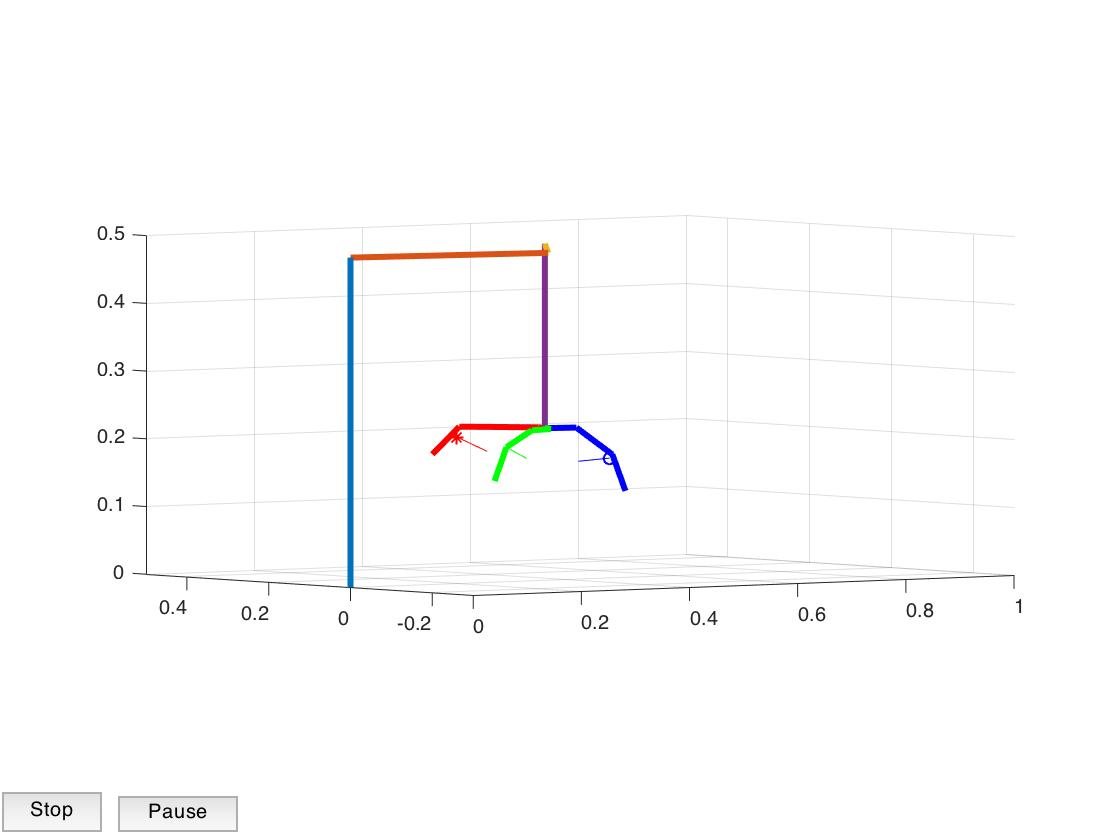
\includegraphics[width=2.5in]{ip.jpg}
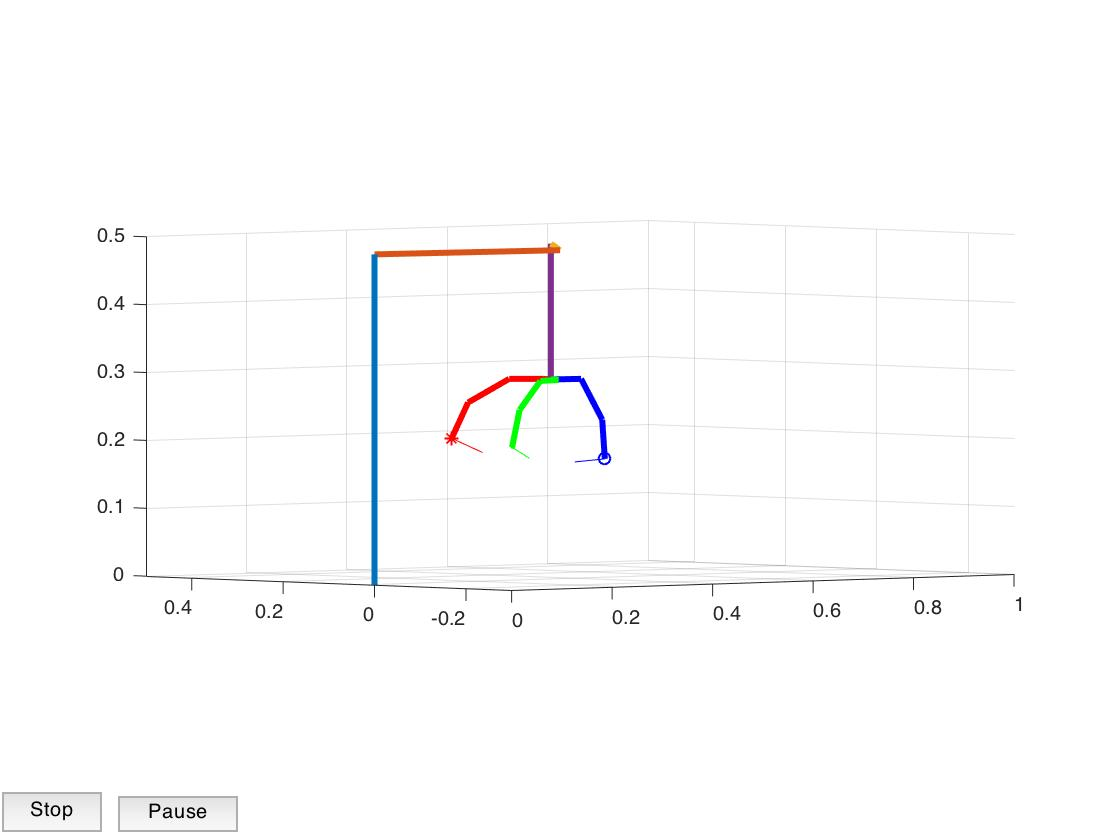
\includegraphics[width=2.5in]{sqp.jpg}
\caption{ First one shows the simulation result by using Interior Point method and second one presents the simulation result by suing SQP method. }
\label{fig_sim }
\end{figure}

\begin{figure}[!t]
\centering
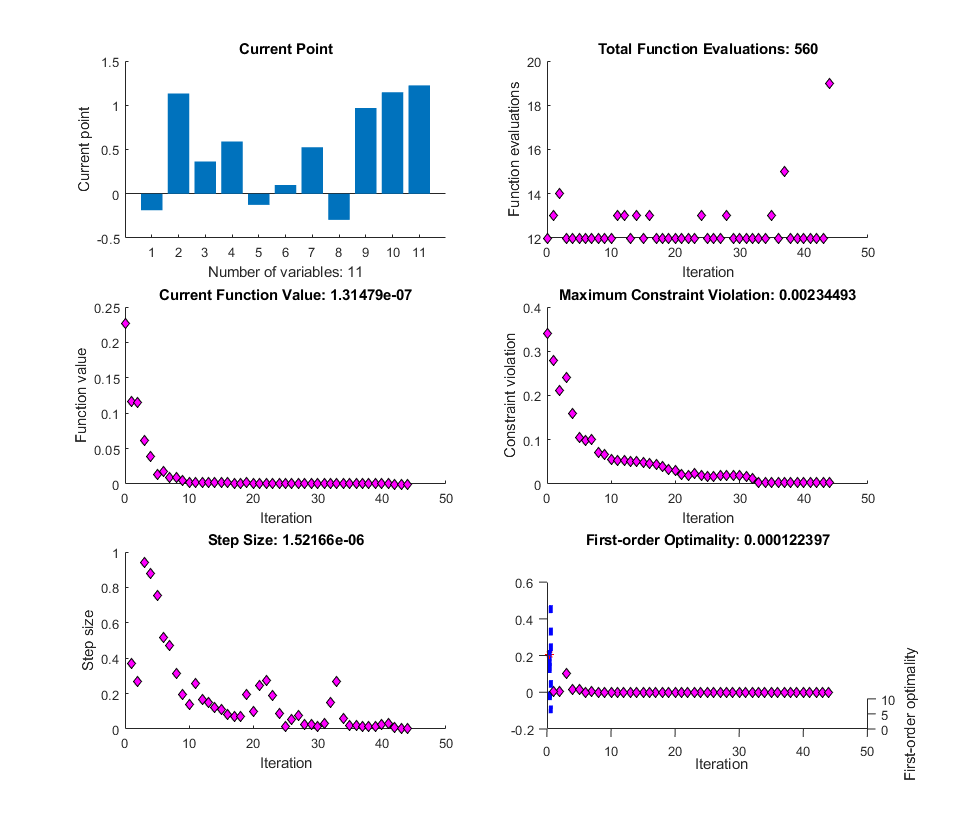
\includegraphics[width=3.5in]{reult.png}
\caption{ Convergence process for the SQP method }
\label{fig_sim }
\end{figure}


\section{Conclusion}
In this project, we solved the inverse kinematics problem for our eight DOF robot system by using nonlinear optimization algorithm. \\
SQP method can always converge to a reasonable destination. Since it does not rely on the inverse of Jacobian matrix, singular points will not effect the solution of it. We also test other nonlinear optimization methods, some of them not convergent and some are quite slow. SQP is stable and fast for solving the inverse kinematics problem for grasping task.  \\






% if have a single appendix:
%\appendix[Proof of the Zonklar Equations]
% or
%\appendix  % for no appendix heading
% do not use \section anymore after \appendix, only \section*
% is possibly needed

% use appendices with more than one appendix
% then use \section to start each appendix
% you must declare a \section before using any
% \subsection or using \label (\appendices by itself
% starts a section numbered zero.)
%


\appendices
\section{Proof of the First Zonklar Equation}
Appendix one text goes here.

% you can choose not to have a title for an appendix
% if you want by leaving the argument blank
\section{}
Appendix two text goes here.


% use section* for acknowledgment
\section*{Acknowledgment}


The authors would like to thank...


% Can use something like this to put references on a page
% by themselves when using endfloat and the captionsoff option.
\ifCLASSOPTIONcaptionsoff
  \newpage
\fi



% trigger a \newpage just before the given reference
% number - used to balance the columns on the last page
% adjust value as needed - may need to be readjusted if
% the document is modified later
%\IEEEtriggeratref{8}
% The "triggered" command can be changed if desired:
%\IEEEtriggercmd{\enlargethispage{-5in}}

% references section

% can use a bibliography generated by BibTeX as a .bbl file
% BibTeX documentation can be easily obtained at:
% http://mirror.ctan.org/biblio/bibtex/contrib/doc/
% The IEEEtran BibTeX style support page is at:
% http://www.michaelshell.org/tex/ieeetran/bibtex/
%\bibliographystyle{IEEEtran}
% argument is your BibTeX string definitions and bibliography database(s)
%\bibliography{IEEEabrv,../bib/paper}
%
% <OR> manually copy in the resultant .bbl file
% set second argument of \begin to the number of references
% (used to reserve space for the reference number labels box)
\begin{thebibliography}{1}

\bibitem{IEEEhowto:kopka}
H.~Kopka and P.~W. Daly, \emph{A Guide to \LaTeX}, 3rd~ed.\hskip 1em plus
  0.5em minus 0.4em\relax Harlow, England: Addison-Wesley, 1999.

\end{thebibliography}

\begin{thebibliography}{2}

\bibitem{IEEEhowto:kopka}
Tomomichi Sugihara, \emph{Solvability-Unconcerned Inverse Kinematics by the Levenberg–Marquardt Method
}\hskip 1em plus
  0.5em minus 0.4em\relax IEEE TRANSACTIONS ON ROBOTICS, VOL. 27, NO. 5, OCTOBER 2011. 

\end{thebibliography}
%Solvability-Unconcerned Inverse Kinematics by the Levenberg–Marquardt Method

% biography section
% 
% If you have an EPS/PDF photo (graphicx package needed) extra braces are
% needed around the contents of the optional argument to biography to prevent
% the LaTeX parser from getting confused when it sees the complicated
% \includegraphics command within an optional argument. (You could create
% your own custom macro containing the \includegraphics command to make things
% simpler here.)
%\begin{IEEEbiography}[{\includegraphics[width=1in,height=1.25in,clip,keepaspectratio]{mshell}}]{Michael Shell}
% or if you just want to reserve a space for a photo:

%\begin{IEEEbiography}{Michael Shell}
%Biography text here.
%\end{IEEEbiography}

% if you will not have a photo at all:
%\begin{IEEEbiographynophoto}{John Doe}
%Biography text here.
%\end{IEEEbiographynophoto}

% insert where needed to balance the two columns on the last page with
% biographies
%\newpage

%\begin{IEEEbiographynophoto}{Jane Doe}
%Biography text here.
%\end{IEEEbiographynophoto}

% You can push biographies down or up by placing
% a \vfill before or after them. The appropriate
% use of \vfill depends on what kind of text is
% on the last page and whether or not the columns
% are being equalized.

%\vfill

% Can be used to pull up biographies so that the bottom of the last one
% is flush with the other column.
%\enlargethispage{-5in}



% that's all folks
\end{document}


